\chapter{Tensor Tracing}\label{chapter:tracer}

\section{The Tracer}\label{sec:tracer-design}

The tracer hooks into llama.cpp's compute path at a single point that every operation crosses, so we capture every operation regardless of operator type.
Only the first worker thread emits a record per operation.
The other threads skip the trace path.

Each record is a fixed-size 1024-byte binary entry carrying the timestamp, the layer and token IDs, the destination tensor name, up to four source tensor descriptors, and the expert IDs for MoE-routed operations.
Each source descriptor labels the source with a memory class: \emph{disk} for the memory-mapped GGUF file (the model weights), or \emph{buffer} for the runtime's anonymous memory (KV cache and scratch).
For disk-backed sources the descriptor also records the GGUF byte offset, so the access can be tied back to the file layout.

Records are written through a thread-local buffer that flushes into a memory-mapped log file, so writes never block compute.
A small Python toolchain converts the binary log into per-token JSON, which feeds the visualizers.

A second, narrower instrumentation stream lives inside our expert buffer manager.
It records the sequence of (layer, projection, expert) cache lookups together with the hit-or-miss outcome of each.
This dump is the input to the offline replacement simulator, which replays it under alternative policies.


\section{What the Trace Reveals}\label{sec:tracer-findings}

Each expert weight matrix on GPT-OSS-20B is 4{,}406{,}400 bytes on disk, or 4.20~MiB.
Of the 12.85~GiB of model weights, 9.48~GiB are expert weights, 1.19~GiB is attention, 1.08~GiB is the output projection, 1.08~GiB is the token embedding, and 8.44~MiB are router weights, one router per layer.

During decode, every read of an expert weight from disk is dereferenced inside the matmul that consumes it.
Under the default loader, that dereference is what triggers the page fault that brings the slice into RAM.

Across 1999 generated tokens, expert selection is far from uniform.
Each MoE layer picks 4 of its 32 experts per token, so a balanced router would select each expert about 250 times over the run.
The actual range is 0 to 1635 selections per (layer, expert) pair, and the imbalance is heavily layer-dependent.
Layer 10 is concentrated: the median expert is picked only 68 times, well below the 250 of a uniform router, while one expert is picked 1635 times (on 81.79\% of tokens).
At layer 0 the routing is closer to uniform: the median is 220 and the most-used expert 589.

\begin{figure}[htbp]
\centering
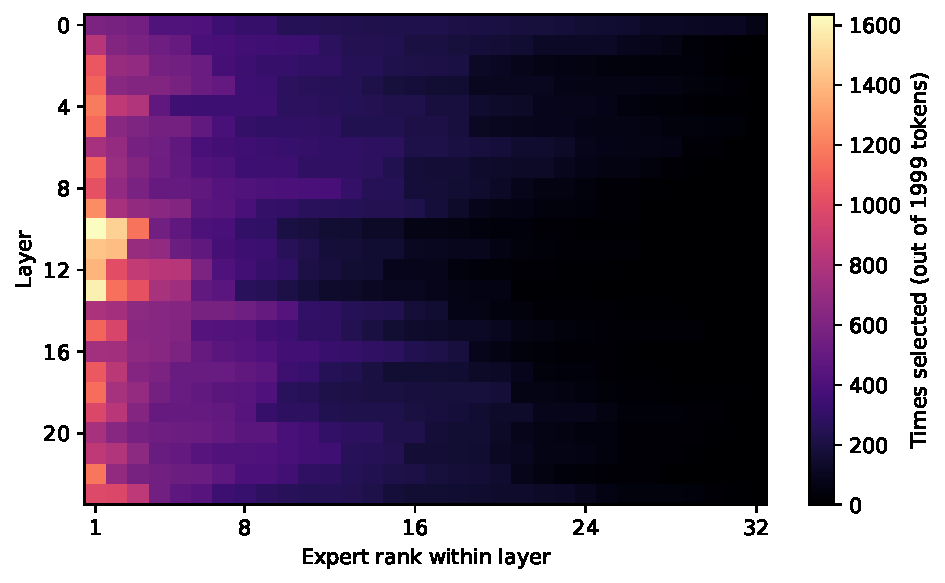
\includegraphics[width=0.85\textwidth]{figures/canon/expert_selection_heatmap.pdf}
\caption[Per-layer expert selection counts]{Selection counts for each (layer, expert) pair across 1999 generated tokens. Within each layer (row), the 32 experts are sorted by selection count descending, so column 1 is the layer's most-selected expert. Layers 10 to 13 fall off steeply (a few experts dominate the rest); layer 0 is much flatter.}
\label{fig:expert-selection-heatmap}
\end{figure}

The temporal access pattern is sharply skewed toward immediate reuse: 45.31\% of (layer, expert) reuses happen at the very next token, 76.14\% within five tokens, and 87.12\% within ten (\autoref{fig:reuse-distance-cdf}).
This is what makes a small in-memory cache effective even when its slot count sits below the per-token working set of 288: the experts that are about to be needed again are usually the ones just used.

\begin{figure}[htbp]
\centering
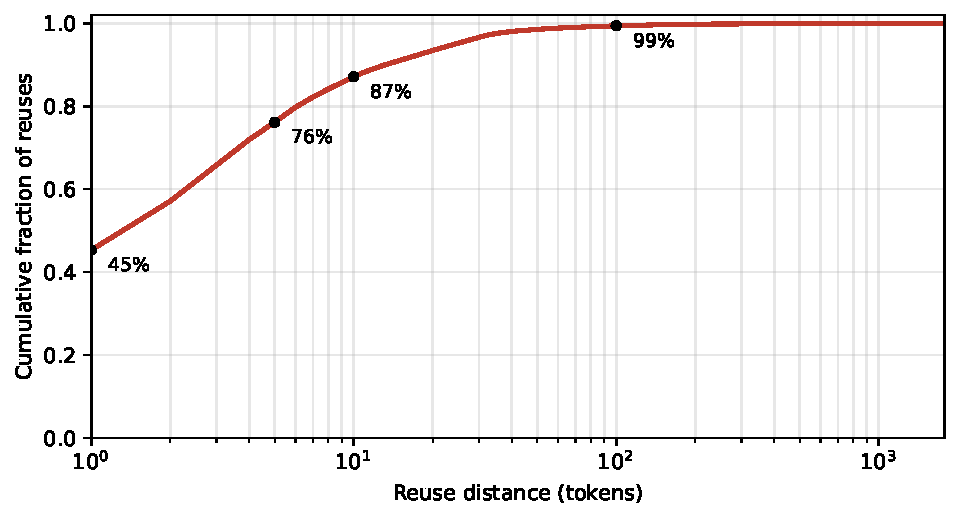
\includegraphics[width=0.85\textwidth]{figures/canon/reuse_distance_cdf.pdf}
\caption[Reuse-distance CDF for (layer, expert) selections]{Reuse distance for (layer, expert) selections in the canonical 1999-token decode. Distance is the number of tokens between two consecutive selections of the same (layer, expert) pair.}
\label{fig:reuse-distance-cdf}
\end{figure}


\section{Visualization}\label{sec:tracer-viz}

Two visualizers consume the per-token JSON.
The first is a browser-based viewer for one or two tokens at a time, with three synchronized views: a per-operation timeline, that token's computation graph, and a heatmap of reads against file offset.
The second is a native desktop application that drops the graph view in exchange for handling a hundred tokens or more, used for analysis across many tokens.


\section{Simulating Replacement}\label{sec:tracer-sim}

The simulator replays the buffer-access dump under five replacement policies and reports the resulting hit rate at a chosen cache size.
We compare LRU, LFU, LFU with periodic counter decay (LFU-aging), Adaptive Replacement Cache (ARC)~\cite{megiddo2003arc}, and W-TinyLFU~\cite{einziger2017tinylfu}.

\begin{table}[htbp]
\centering
\caption[Cache hit rate by policy and cache size]{Cache hit rate by replacement policy and cache size on the canonical 20B trace (1999 tokens, 575{,}724 expert weight accesses). The per-token working set is 288 slices. Bold marks the best policy at each cache size.}
\label{tab:tracer-policy-hits}
\begin{tabular}{lrrrrr}
\toprule
Cache slots & LRU & LFU & LFU-aging & ARC & W-TinyLFU \\
\midrule
200  &  0.00\% & 13.36\% & \textbf{29.08\%} &  0.00\% & 25.21\% \\
250  &  0.00\% & 16.85\% & \textbf{34.13\%} &  0.00\% & 31.05\% \\
288  & \textbf{36.02\%} & 19.47\% & 30.48\% & 32.92\% & 33.33\% \\
400  & 46.31\% & 28.97\% & 46.11\% & \textbf{48.04\%} & 42.39\% \\
500  & 54.88\% & 33.70\% & 54.03\% & \textbf{56.32\%} & 50.30\% \\
750  & 73.32\% & 46.77\% & 68.47\% & \textbf{73.68\%} & 70.40\% \\
1000 & 85.36\% & 62.02\% & 79.83\% & \textbf{85.46\%} & 77.46\% \\
\bottomrule
\end{tabular}
\end{table}

\begin{figure}[htbp]
\centering
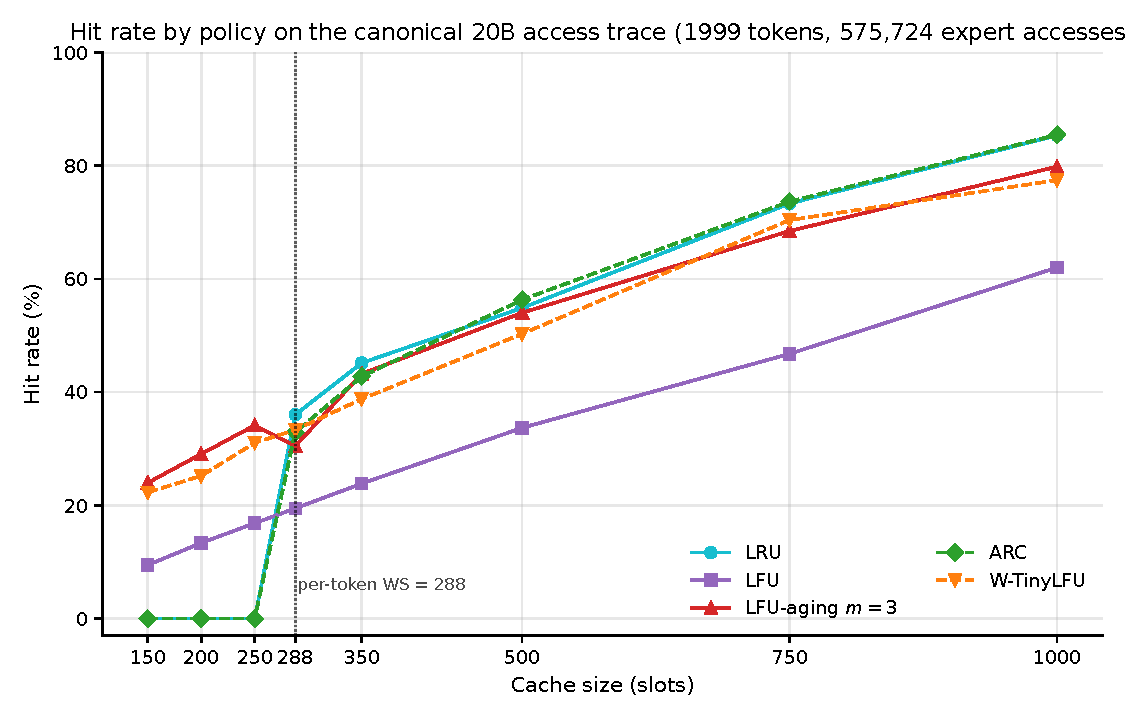
\includegraphics[width=0.85\textwidth]{figures/canon/lfu_lru_crossover.pdf}
\caption[Simulator hit rate by policy across cache sizes]{Simulator hit-rate curves on the canonical 20B trace, sweeping cache sizes from 150 to 1000 slots. The dotted vertical line marks the per-token working set of 288 slices, where the regime crossover happens: below it, LRU and ARC drop to zero while LFU-aging dominates; above it, LRU and ARC recover and lead.}
\label{fig:lfu-lru-crossover}
\end{figure}

The cache size relative to the per-token working set of 288 slices determines which policy wins.
Below the working set (200 and 250 slots), LRU and ARC produce zero hits: by the time a slice is selected for the second time, LRU has already evicted it, because the recency tail is exactly what is needed next.
LFU-aging dominates this regime by holding on to the small set of frequently-routed-to experts.
At and above the working set, LRU recovers, because the cache fits a token's reads with room to spare and per-access recency tracking now captures the immediate reuses of \autoref{fig:reuse-distance-cdf}.
LFU's counters suffer from stale popularity: experts that were heavily selected earlier in the run hold on to their slots after they have cooled.
ARC tracks LRU within a percentage point at every cache size where it is non-zero, and W-TinyLFU sits between the two extremes.

The simulator's LFU-aging implementation reproduces the hit rate of the deployed C runtime to within rounding (34.13\% simulated, 33.80\% measured at the canonical 7~GiB / 250-slot configuration), so the rankings in \autoref{tab:tracer-policy-hits} reflect what the runtime would observe.
The aging period was tuned on the simulator: counters are halved every $3 \times \mathit{cache\_slots}$ accesses, the highest-hit-rate multiplier we tested.
Routing-aware prefetching, which predicts the next layer's experts so their slices can be read ahead of time, is an active research direction~\cite{jia2025activeflow,xue2024moeinfinity} and is out of scope here.
